% !TEX TS-program = XeLaTeX
% !TEX encoding = UTF-8 Unicode

\chapter{需求分析}
\label{chap07}
\defaultfont
~\\
\section{可行性分析}
~\\
\subsection{技术可行性分析}
\subsection{经济可行性分析}
\subsection{操作可行性分析}
~\\
\section{业务流程分析}

 (1) 管理员通过教职员学生管理系统与论文评审评分系统联动导入学生,教师信息。

(2) 学生上传论文

学生上传论文,待评审导师进行检查。

(3) 检查论文

教师检查论文,若论文未达到审批要求,教师可进行留言并贴上缺陷标签,待学生修改论文并重新上传论文。

(4) 论文打分

若论文达到审批要求,教师可对论文进行打分。

(5) 统计得分情况

管理员可查看所有学生论文得分比例。

(5) 统计教师评审量,评审情况

管理员可查看各个教师总评审量,已完成评审比例,供后续任务量分配做参考。

(6) 统计论文中出现的问题

管理可查看所有缺陷标签以及标签引用量。
\begin{figure}[h]
	\centering
	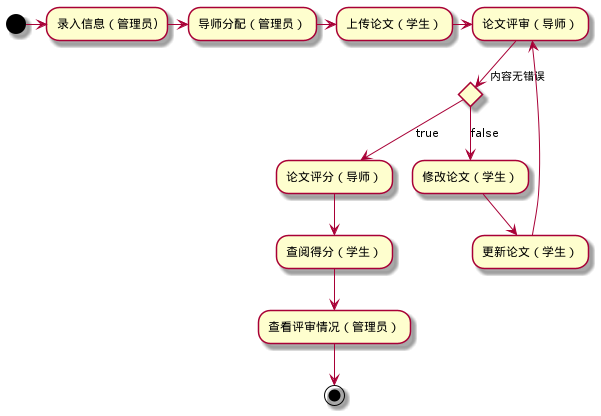
\includegraphics[scale = 0.6]{out/uml/流程图/系统总体活动流程图/系统总体活动流程图.png}
	\caption{\song\wuhao 系统总体活动流程图}
\end{figure}


\section{系统功能需求分析}

\subsection{系统总体功能}

\begin{figure}[h]
	\centering
	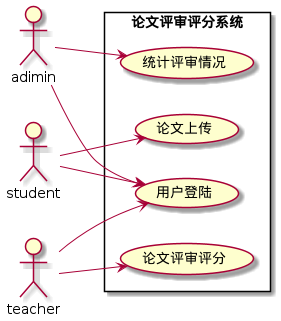
\includegraphics[scale = 0.6]{out/uml/用例图/系统总体功能用例图/系统总体功能用例图.png}
	\caption{\song\wuhao 系统总体功能用例图}
\end{figure}

\subsection{用户登录}

\begin{figure}[h]
	\centering
	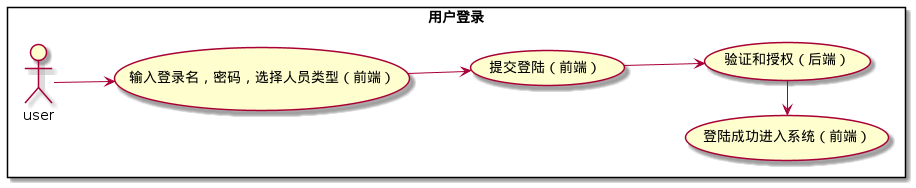
\includegraphics[scale = 0.5]{out/uml/用例图/1-用户登录用例图/1-用户登录用例图.png}
	\caption{\song\wuhao 用户登录用例图}
\end{figure}

\subsection{论文上传}

\begin{figure}[h]
	\centering
	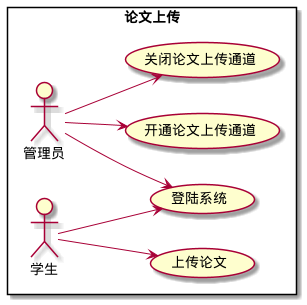
\includegraphics[scale = 0.6]{out/uml/用例图/2-论文上传/2-论文上传.png}
	\caption{\song\wuhao 论文上传}
\end{figure}

\subsection{论文评审评分}

\begin{figure}[h]
	\centering
	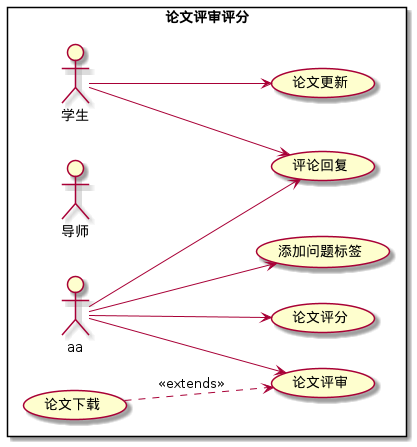
\includegraphics[scale = 0.6]{out/uml/用例图/3-论文评审评分/3-论文评审评分.png}
	\caption{\song\wuhao 论文评审评分}
\end{figure}

\subsection{统计评审情况}

\begin{figure}[h]
	\centering
	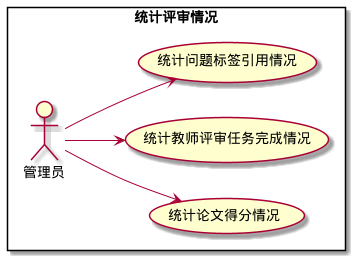
\includegraphics[scale = 0.6]{out/uml/用例图/4-统计评审情况/4-统计评审情况.png}
	\caption{\song\wuhao 统计评审情况}
\end{figure}
